% questions.tex —— 2007 年·普通高等学校招生考试·新课标卷·文科 · 题目内容片段（无答案）
% 由 tools/generate_projects.py 依来源总账自 2007/2007_数学真题_新课标文_试题.md 生成，勿手改（改源 MD 后重跑）


状态：needs-review；依固定候选 PDF 两页（印刷页 395–396）三栏图像以 300 dpi 渲染逐题核验，图形已矢量重绘，正式构建与逐页验收待完成。源未列各题分值，不补分值。

\gkpart{一、选择题}

\begin{question}
\gkti{1}设集合 $A=\{x\mid x>-1\}$，$B=\{x\mid -2<x<2\}$，则 $A\cup B=$（　）

（A）$\{x\mid x>-2\}$

（B）$\{x\mid x>-1\}$

（C）$\{x\mid -2<x<-1\}$

（D）$\{x\mid -1<x<2\}$

\end{question}
\begin{question}
\gkti{2}已知命题 $p$：$\forall x\in\mathbf R$，$\sin x\leqslant1$，则（　）

（A）$\neg p$：$\exists x\in\mathbf R$，$\sin x\geqslant1$

（B）$\neg p$：$\forall x\in\mathbf R$，$\sin x\geqslant1$

（C）$\neg p$：$\exists x\in\mathbf R$，$\sin x>1$

（D）$\neg p$：$\forall x\in\mathbf R$，$\sin x>1$

\Needspace{0.4\textheight}
\end{question}
\begin{question}
\gkti{3}函数 $y=\sin\left(2x-\dfrac{\pi}{3}\right)$ 在区间 $\left[-\dfrac{\pi}{2},\pi\right]$ 的简图是（　）
\nopagebreak[4]
\begin{center}% 2007 年新课标卷文科第 3 题：函数 y=sin(2x-π/3) 在 [-π/2,π] 上的四个简图选项。
%   （A）为正确图象；（B）（C）（D）为相位不同的干扰项。
% 来源 PDF：gaokaomath-src/普通高考/2007/2007新课标文(海南,宁夏).pdf
% SHA-256：c8ee1632ac3a7a28aab1150f047a2e1c74398ca2944701e9165237897ae724e2
% 原页：2007新课标文(海南,宁夏).pdf 第 1 页（A3 三栏）第 1 栏，书页码 393。
% 重绘依据：按原页四个小图的零点、极值位置与坐标轴标注重绘；横轴以 π 为单位。
\begin{tikzpicture}[x=2.6cm, y=1.6cm, semithick,
  every node/.style={inner sep=1pt, font=\small}]

  % ================= （A）正确图象 =================
  \begin{scope}[shift={(0cm,0cm)}]
    \draw[->,>=stealth] (-0.66,0) -- (1.20,0) node[right] {$x$};
    \draw[->,>=stealth] (0,-1.22) -- (0,1.38) node[above] {$y$};
    \draw[domain=-0.5:1,samples=200,line width=1pt]
      plot (\x,{sin(deg(2*pi*\x - pi/3))});
    \draw[dashed] (-0.5,0) -- (-0.5,{sin(deg(-pi - pi/3))});
    \draw[dashed] (1,0) -- (1,{sin(deg(2*pi - pi/3))});
    \node[below] at (-0.5,0) {$-\frac{\pi}{2}$};
    \node[below left=1pt] at (0,0) {$O$};
    \node[below] at (1,0) {$\pi$};
    \node[left=2pt] at (0,1) {$1$};
    \node[left=2pt] at (0,-1) {$-1$};
    \node[below] at (0.55,-1.55) {（A）};
  \end{scope}

  % ================= （B） =================
  \begin{scope}[shift={(7.2cm,0cm)}]
    \draw[->,>=stealth] (-0.66,0) -- (1.20,0) node[right] {$x$};
    \draw[->,>=stealth] (0,-1.22) -- (0,1.38) node[above] {$y$};
    \draw[domain=-0.5:1,samples=200,line width=1pt]
      plot (\x,{sin(deg(2*pi*\x + pi/3))});
    \draw[dashed] (-0.5,0) -- (-0.5,{sin(deg(-pi + pi/3))});
    \draw[dashed] (1,0) -- (1,{sin(deg(2*pi + pi/3))});
    \node[below] at (-0.5,0) {$-\frac{\pi}{2}$};
    \node[below left=1pt] at (0,0) {$O$};
    \node[below] at (1,0) {$\pi$};
    \node[left=2pt] at (0,1) {$1$};
    \node[left=2pt] at (0,-1) {$-1$};
    \node[below] at (0.55,-1.55) {（B）};
  \end{scope}

  % ================= （C） =================
  \begin{scope}[shift={(0cm,-5.35cm)}]
    \draw[->,>=stealth] (-0.66,0) -- (1.20,0) node[right] {$x$};
    \draw[->,>=stealth] (0,-1.22) -- (0,1.38) node[above] {$y$};
    \draw[domain=-0.5:1,samples=200,line width=1pt]
      plot (\x,{sin(deg(2*pi*\x - 2*pi/3))});
    \draw[dashed] (-0.5,0) -- (-0.5,{sin(deg(-pi - 2*pi/3))});
    \draw[dashed] (1,0) -- (1,{sin(deg(2*pi - 2*pi/3))});
    \node[below] at (-0.5,0) {$-\frac{\pi}{2}$};
    \node[below left=1pt] at (0,0) {$O$};
    \node[below] at (1,0) {$\pi$};
    \node[left=2pt] at (0,1) {$1$};
    \node[left=2pt] at (0,-1) {$-1$};
    \node[below] at (0.55,-1.55) {（C）};
  \end{scope}

  % ================= （D） =================
  \begin{scope}[shift={(7.2cm,-5.35cm)}]
    \draw[->,>=stealth] (-0.66,0) -- (1.20,0) node[right] {$x$};
    \draw[->,>=stealth] (0,-1.22) -- (0,1.38) node[above] {$y$};
    \draw[domain=-0.5:1,samples=200,line width=1pt]
      plot (\x,{sin(deg(2*pi*\x + 2*pi/3))});
    \draw[dashed] (-0.5,0) -- (-0.5,{sin(deg(-pi + 2*pi/3))});
    \draw[dashed] (1,0) -- (1,{sin(deg(2*pi + 2*pi/3))});
    \node[below] at (-0.5,0) {$-\frac{\pi}{2}$};
    \node[below left=1pt] at (0,0) {$O$};
    \node[below] at (1,0) {$\pi$};
    \node[left=2pt] at (0,1) {$1$};
    \node[left=2pt] at (0,-1) {$-1$};
    \node[below] at (0.55,-1.55) {（D）};
  \end{scope}
\end{tikzpicture}
\end{center}
\nopagebreak[4]
\end{question}
\begin{question}
\gkti{4}已知平面向量 $\boldsymbol a=(1,1)$，$\boldsymbol b=(1,-1)$，则向量 $\dfrac12\boldsymbol a-\dfrac32\boldsymbol b=$（　）

（A）$(-2,-1)$

（B）$(-2,1)$

（C）$(-1,0)$

（D）$(-1,2)$

\Needspace{0.4\textheight}
\end{question}
\begin{question}
\gkti{5}如果执行下面的程序框图，那么输出的 $S=$（　）
\nopagebreak[4]
\begin{center}% 2007 年新课标卷文科第 5 题：程序框图（k 从 1 到 50 累加 2k）。
% 来源 PDF：gaokaomath-src/普通高考/2007/2007新课标文(海南,宁夏).pdf
% SHA-256：c8ee1632ac3a7a28aab1150f047a2e1c74398ca2944701e9165237897ae724e2
% 原页：2007新课标文(海南,宁夏).pdf 第 1 页（A3 三栏）第 1 栏，书页码 393。
% 重绘依据：按原页流程与分支方向重绘；循环体为 S=S+2k、k=k+1。
\begin{tikzpicture}[scale=1.0, semithick,
  every node/.style={inner sep=2pt},
  box/.style={draw, rounded corners=2pt, minimum width=1.9cm,
    minimum height=0.55cm, align=center},
  para/.style={draw, trapezium, trapezium left angle=70,
    trapezium right angle=110, minimum width=2.4cm, minimum height=0.55cm,
    align=center},
  dec/.style={draw, diamond, aspect=2.4, minimum width=2.8cm,
    minimum height=1.1cm, align=center},
  arr/.style={->, >=stealth}]

  \node[box]  (start) at (0,7.2) {开始};
  \node[box]  (init)  at (0,6.3) {$k=1$};
  \node[box]  (sum)   at (0,5.4) {$S=0$};
  \node[dec]  (test)  at (0,4.2) {$k\leqslant50$?};
  \node[box]  (add)   at (0,2.95) {$S=S+2k$};
  \node[box]  (inc)   at (0,2.15) {$k=k+1$};
  \node[para] (out)   at (4.6,4.2) {输出 $S$};
  \node[box]  (end)   at (4.6,3.3) {结束};

  \draw[arr] (start) -- (init);
  \draw[arr] (init) -- (sum);
  \draw[arr] (sum) -- (test);
  \draw[arr] (test.south) -- node[left] {是} (add.north);
  \draw[arr] (add) -- (inc);
  \draw[arr] (inc.west) -- (-2.5,2.15) -- (-2.5,4.75) -- (0,4.75);
  \draw[arr] (test.east) -- node[above] {否} (out.west);
  \draw[arr] (out) -- (end);
\end{tikzpicture}
\end{center}
\nopagebreak[4]
（A）$2450$

（B）$2500$

（C）$2550$

（D）$2652$

\end{question}
\begin{question}
\gkti{6}已知 $a$，$b$，$c$，$d$ 成等比数列，且曲线 $y=x^2-2x+3$ 的顶点是 $(b,c)$，则 $ad$ 等于（　）

（A）$3$

（B）$2$

（C）$1$

（D）$-2$

\end{question}
\begin{question}
\gkti{7}已知抛物线 $y^2=2px$（$p>0$）的焦点为 $F$，点 $P_1(x_1,y_1)$，$P_2(x_2,y_2)$，$P_3(x_3,y_3)$ 在抛物线上，且 $2x_2=x_1+x_3$，则有（　）

（A）$|FP_1|+|FP_2|=|FP_3|$

（B）$|FP_1|^2+|FP_2|^2=|FP_3|^2$

（C）$2|FP_2|=|FP_1|+|FP_3|$

（D）$|FP_2|^2=|FP_1|\cdot|FP_3|$

\Needspace{0.4\textheight}
\end{question}
\begin{question}
\gkti{8}已知某个几何体的三视图如下，根据图中标出的尺寸（单位：$\mathrm{cm}$），可得这个几何体的体积是（　）
\nopagebreak[4]
\begin{center}% 2007 年新课标卷文科第 8 题：三视图（正视图、侧视图、俯视图）及尺寸。
%   正视图为直角边 20、20 的直角三角形；侧视图为底边 20、高 20 的等腰三角形；
%   俯视图为 20×20 正方形并画对角线，右侧标注 10 与 10。
% 来源 PDF：gaokaomath-src/普通高考/2007/2007新课标文(海南,宁夏).pdf
% SHA-256：c8ee1632ac3a7a28aab1150f047a2e1c74398ca2944701e9165237897ae724e2
% 原页：2007新课标文(海南,宁夏).pdf 第 1 页（A3 三栏）第 2 栏，书页码 393。
% 重绘依据：按原页三个视图的位置、形状与尺寸标注重绘，单位 cm。
\begin{tikzpicture}[x=0.115cm, y=0.095cm, semithick,
  every node/.style={inner sep=1.5pt, font=\small}]

  % ---------------- 正视图 ----------------
  \begin{scope}[shift={(0cm,0cm)}]
    \draw (0,0) -- (20,0) -- (20,20) -- cycle;
    % 尺寸 20（下）
    \draw[<->,>=stealth] (0,-4) -- (20,-4);
    \draw (0,-1.5) -- (0,-5.5);
    \draw (20,-1.5) -- (20,-5.5);
    \node[below] at (10,-4) {$20$};
    % 尺寸 20（右）
    \draw[<->,>=stealth] (24,0) -- (24,20);
    \draw (22,0) -- (26,0);
    \draw (22,20) -- (26,20);
    \node[right] at (24,10) {$20$};
    \node[below] at (10,-9) {正视图};
  \end{scope}

  % ---------------- 侧视图 ----------------
  \begin{scope}[shift={(3.6cm,0cm)}]
    \draw (0,0) -- (20,0) -- (10,20) -- cycle;
    \draw[<->,>=stealth] (0,-4) -- (20,-4);
    \draw (0,-1.5) -- (0,-5.5);
    \draw (20,-1.5) -- (20,-5.5);
    \node[below] at (10,-4) {$20$};
    \node[below] at (10,-9) {侧视图};
  \end{scope}

  % ---------------- 俯视图 ----------------
  \begin{scope}[shift={(0.9cm,-3.6cm)}]
    \draw (0,0) rectangle (20,20);
    \draw (0,0) -- (20,20);
    \draw (0,20) -- (20,0);
    % 尺寸 20（下）
    \draw[<->,>=stealth] (0,-4) -- (20,-4);
    \draw (0,-1.5) -- (0,-5.5);
    \draw (20,-1.5) -- (20,-5.5);
    \node[below] at (10,-4) {$20$};
    % 右侧 10 与 10
    \draw[<->,>=stealth] (24,0) -- (24,10);
    \draw[<->,>=stealth] (24,10) -- (24,20);
    \draw (22,0) -- (26,0);
    \draw (22,10) -- (26,10);
    \draw (22,20) -- (26,20);
    \node[right] at (24,5) {$10$};
    \node[right] at (24,15) {$10$};
    \node[below] at (10,-9) {俯视图};
  \end{scope}
\end{tikzpicture}
\end{center}
\nopagebreak[4]
（A）$\dfrac{4000}{3}\ \mathrm{cm^3}$

（B）$\dfrac{8000}{3}\ \mathrm{cm^3}$

（C）$2000\ \mathrm{cm^3}$

（D）$4000\ \mathrm{cm^3}$

\end{question}
\begin{question}
\gkti{9}若 $\dfrac{\cos2\alpha}{\sin\left(\alpha-\dfrac{\pi}{4}\right)}=-\dfrac{\sqrt2}{2}$，则 $\cos\alpha+\sin\alpha$ 的值为（　）

（A）$-\dfrac{\sqrt7}{2}$

（B）$-\dfrac12$

（C）$\dfrac12$

（D）$\dfrac{\sqrt7}{2}$

\end{question}
\begin{question}
\gkti{10}曲线 $y=\mathrm e^x$ 在点 $(2,\mathrm e^2)$ 处的切线与坐标轴所围三角形的面积为（　）

（A）$\dfrac94\mathrm e^2$

（B）$2\mathrm e^2$

（C）$\mathrm e^2$

（D）$\dfrac{\mathrm e^2}{2}$

\end{question}
\begin{question}
\gkti{11}已知三棱锥 $S-ABC$ 的各顶点都在一个半径为 $r$ 的球面上，球心 $O$ 在 $AB$ 上，$SO\perp$ 底面 $ABC$，$AC=\sqrt2r$，则球的体积与三棱锥体积之比是（　）

（A）$\pi$

（B）$2\pi$

（C）$3\pi$

（D）$4\pi$

\end{question}
\begin{question}
\gkti{12}甲、乙、丙三名射箭运动员在某次测试中各射箭 $20$ 次，三人的测试成绩如下表

\begin{center}
\begin{tabular}{llllll}
\toprule
运动员 & 环数 & $7$ & $8$ & $9$ & $10$ \\
\midrule
甲 & 频数 & $5$ & $5$ & $5$ & $5$ \\
乙 & 频数 & $6$ & $4$ & $4$ & $6$ \\
丙 & 频数 & $4$ & $6$ & $6$ & $4$ \\
\bottomrule
\end{tabular}
\end{center}

$s_1$，$s_2$，$s_3$ 分别表示甲、乙、丙三名运动员这次测试成绩的标准差，则有（　）

（A）$s_3>s_1>s_2$

（B）$s_2>s_1>s_3$

（C）$s_1>s_2>s_3$

（D）$s_2>s_3>s_1$

\end{question}
\gkpart{二、填空题}

\begin{question}
\gkti{13}已知双曲线的顶点到渐近线的距离为 $2$，焦点到渐近线的距离为 $6$，则该双曲线的离心率为\gkblank{}。

\end{question}
\begin{question}
\gkti{14}设函数 $f(x)=(x+1)(x+a)$ 为偶函数，则 $a=$\gkblank{}。

\end{question}
\begin{question}
\gkti{15}$\mathrm i$ 是虚数单位，$\mathrm i+2\mathrm i^2+3\mathrm i^3+\cdots+8\mathrm i^8=$\gkblank{}。（用 $a+b\mathrm i$ 的形式表示，$a$，$b\in\mathbf R$）

\end{question}
\begin{question}
\gkti{16}已知 $\{a_n\}$ 是等差数列，$a_4+a_6=6$，其前 $5$ 项和 $S_5=10$，则其公差 $d=$\gkblank{}。

\end{question}
\gkpart{三、解答题}

\Needspace{0.4\textheight}
\begin{question}
\gkti{17}如图，测量河对岸的塔高 $AB$ 时，可以选与塔底 $B$ 在同一水平面内的两个测点 $C$ 与 $D$。现测得 $\angle BCD=\alpha$，$\angle BDC=\beta$，$CD=s$，并在点 $C$ 测得塔顶 $A$ 的仰角为 $\theta$，求塔高 $AB$。
\nopagebreak[4]
\begin{center}% 2007 年新课标卷文科第 17 题：河对岸塔高 AB 的测量示意图。
%   C、D 在同一水平面内的近岸，B 为塔底（对岸），AB 为塔高；
%   A—C、A—D 为视线（虚线），C—D 为近岸基线，B—C、B—D 为水平距离。
% 来源 PDF：gaokaomath-src/普通高考/2007/2007新课标文(海南,宁夏).pdf
% SHA-256：c8ee1632ac3a7a28aab1150f047a2e1c74398ca2944701e9165237897ae724e2
% 原页：2007新课标文(海南,宁夏).pdf 第 1 页（A3 三栏）第 3 栏，书页码 393。
% 重绘依据：按原页塔、河岸、测点与视线的相对位置重绘，尺寸关系不按比例。
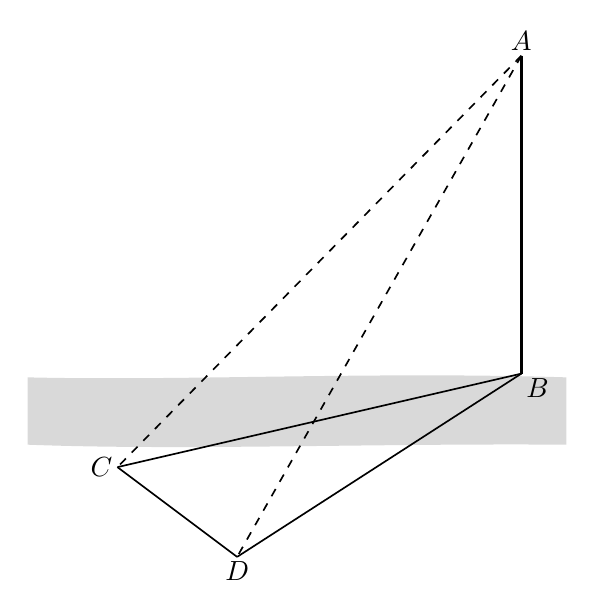
\begin{tikzpicture}[scale=0.95, semithick,
  every node/.style={inner sep=1.5pt}]

  \coordinate (B) at (4.0,0.95);
  \coordinate (A) at (4.0,5.2);
  \coordinate (C) at (-1.4,-0.3);
  \coordinate (D) at (0.2,-1.5);

  % 河面（近岸与对岸之间的灰色带）
  \fill[gray!30]
    (-2.6,0.0) .. controls (-0.5,-0.08) and (2.0,0.02) .. (4.6,0.0)
    -- (4.6,0.9) .. controls (2.0,0.98) and (-0.5,0.85) .. (-2.6,0.9) -- cycle;

  % 塔
  \draw[line width=1.1pt] (A) -- (B);
  \node[above] at (A) {$A$};
  \node[below right] at (B) {$B$};

  % 水平基线与视线
  \draw (C) -- (D);
  \draw (B) -- (C);
  \draw (B) -- (D);
  \draw[dashed] (A) -- (C);
  \draw[dashed] (A) -- (D);

  \node[left] at (C) {$C$};
  \node[below] at (D) {$D$};
\end{tikzpicture}
\end{center}
\nopagebreak[4]
\Needspace{0.4\textheight}
\end{question}
\begin{question}
\gkti{18}如图，$A$，$B$，$C$，$D$ 为空间四点。在 $\triangle ABC$ 中，$AB=2$，$AC=BC=\sqrt2$，等边三角形 $ADB$ 以 $AB$ 为轴运动。

（1）当平面 $ADB\perp$ 平面 $ABC$ 时，求 $CD$；

（2）当 $\triangle ADB$ 转动时，是否总有 $AB\perp CD$？证明你的结论。
\nopagebreak[4]
\begin{center}% 2007 年新课标卷文科第 18 题：空间四点 A、B、C、D，△ADB 以 AB 为轴转动。
%   D 为顶点，A、B 为轴的两端，C 为底面点；AB 被面 DBC 遮挡，画虚线。
% 来源 PDF：gaokaomath-src/普通高考/2007/2007新课标文(海南,宁夏).pdf
% SHA-256：920ab7ed3244ae8c738e34446fd4135b3a5c50c71fb5e03c3eba0f8a7cbcf804
% 原页：2007新课标文(海南,宁夏).pdf 第 1 页（A3 三栏）第 3 栏，书页码 395。
% 重绘依据：按原页 D、A、B、C 的相对位置与虚实线重绘。
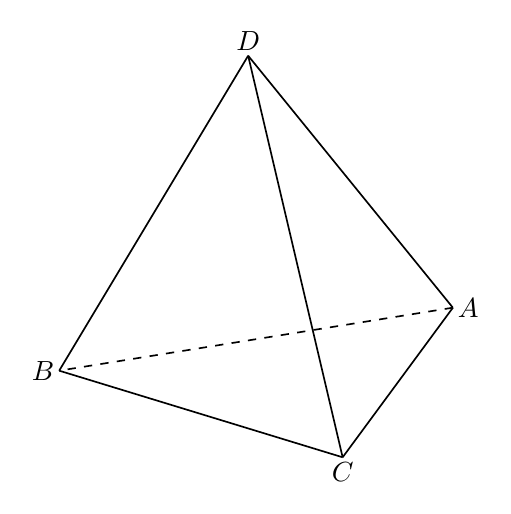
\begin{tikzpicture}[scale=1.0, semithick,
  every node/.style={inner sep=1.5pt}]

  \coordinate (D) at (0,4.0);
  \coordinate (A) at (2.6,0.8);
  \coordinate (B) at (-2.4,0.0);
  \coordinate (C) at (1.2,-1.1);

  \draw (D) -- (A);
  \draw (D) -- (B);
  \draw (D) -- (C);
  \draw (A) -- (C);
  \draw (B) -- (C);
  \draw[dashed] (A) -- (B);

  \node[above] at (D) {$D$};
  \node[right] at (A) {$A$};
  \node[left] at (B) {$B$};
  \node[below] at (C) {$C$};
\end{tikzpicture}
\end{center}
\nopagebreak[4]
\end{question}
\begin{question}
\gkti{19}设函数 $f(x)=\ln(2x+3)+x^2$。

（1）讨论 $f(x)$ 的单调性；

（2）求 $f(x)$ 在区间 $\left[-\dfrac34,\dfrac14\right]$ 的最大值和最小值。

\end{question}
\begin{question}
\gkti{20}设有关于 $x$ 的一元二次方程 $x^2+2ax+b^2=0$。

（1）若 $a$ 是从 $0$，$1$，$2$，$3$ 四个数中任取的一个数，$b$ 是从 $0$，$1$，$2$ 三个数中任取的一个数，求上述方程有实根的概率；

（2）若 $a$ 是从区间 $[0,3]$ 任取的一个数，$b$ 是从区间 $[0,2]$ 任取的一个数，求上述方程有实根的概率。

\end{question}
\begin{question}
\gkti{21}在平面直角坐标系 $xOy$ 中，已知圆 $x^2+y^2-12x+32=0$ 的圆心为 $Q$，过点 $P(0,2)$ 且斜率为 $k$ 的直线与圆 $Q$ 相交于不同的交点 $A$，$B$。

（1）求 $k$ 的取值范围；

（2）是否存在常数 $k$，使得向量 $\overrightarrow{OA}+\overrightarrow{OB}$ 与 $\overrightarrow{PQ}$ 共线？如果存在，求 $k$ 值；如果不存在，请说明理由。

\Needspace{0.4\textheight}
\end{question}
\begin{question}
\gkti{22}如图，已知 $AP$ 是 $\odot O$ 的切线，$P$ 为切点，$AC$ 是 $\odot O$ 的割线，与 $\odot O$ 交于 $B$，$C$ 两点，圆心 $O$ 在 $\angle PAC$ 的内部，点 $M$ 是 $BC$ 的中点。

（1）证明 $A$，$P$，$O$，$M$ 四点共圆；

（2）求 $\angle OAM+\angle APM$ 的大小。
\nopagebreak[4]
\begin{center}% 2007 年新课标卷文科第 22 题：圆的切线 AP、割线 ABC、弦 BC 中点 M。
%   圆 O 半径 2，A(-4,0)，切点 P=(-1,√3)；
%   割线 ABC 从 A 出发，B、C 为与圆的交点，M 为 BC 中点。
% 来源 PDF：gaokaomath-src/普通高考/2007/2007新课标文(海南,宁夏).pdf
% SHA-256：c8ee1632ac3a7a28aab1150f047a2e1c74398ca2944701e9165237897ae724e2
% 原页：2007新课标文(海南,宁夏).pdf 第 2 页（A3 三栏）第 3 栏，书页码 394。
% 重绘依据：按原页点、线与圆的位置重绘；A-O 与 P-M 为题目用到的辅助线。
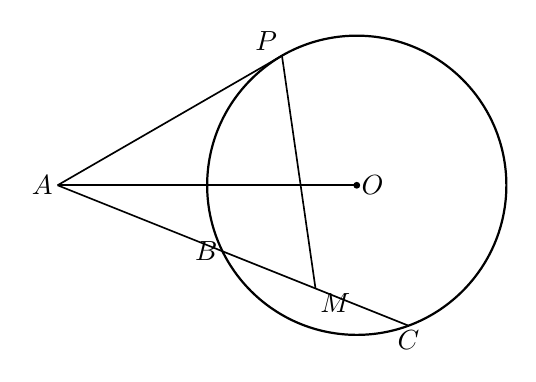
\begin{tikzpicture}[scale=0.95, semithick,
  every node/.style={inner sep=1.5pt}]

  \coordinate (O) at (0,0);
  \coordinate (A) at (-4,0);
  \coordinate (P) at (-1,1.732);
  \coordinate (B) at (-1.795,-0.882);
  \coordinate (C) at (0.692,-1.877);
  \coordinate (M) at (-0.5515,-1.3795);

  \draw[thick] (O) circle (2);
  \fill (O) circle (1.3pt);

  % 切线、割线与辅助线
  \draw (A) -- (P);
  \draw (A) -- (C);
  \draw (A) -- (O);
  \draw (P) -- (M);

  \node[left] at (A) {$A$};
  \node[above left] at (P) {$P$};
  \node[right] at (O) {$O$};
  \node[left] at (B) {$B$};
  \node[below] at (C) {$C$};
  \node[below right] at (M) {$M$};
\end{tikzpicture}
\end{center}
\nopagebreak[4]
\end{question}
\gkpart{四、选做题}

\begin{question}
\gkti{23}$\odot O_1$ 和 $\odot O_2$ 的极坐标方程分别为 $\rho=4\cos\theta$，$\rho=-4\sin\theta$。

（1）把 $\odot O_1$ 和 $\odot O_2$ 的极坐标方程化为直角坐标方程；

（2）求经过 $\odot O_1$，$\odot O_2$ 交点的直线的直角坐标方程。

\end{question}
\begin{question}
\gkti{24}设函数 $f(x)=|2x+1|-|x-4|$。

（1）解不等式 $f(x)>2$；

（2）求函数 $y=f(x)$ 的最小值。

\end{question}